Desde el inicio del proyecto, los integrantes del equipo han mostrado un gran interés
y ganas de desarrollar este proyecto. La idea inicial se planteó como un robot
impreso en 3D que pudiera resultar accesible para cualquiera, a partir de lo estudiado
y visto en la asignatura de Robótica del grado de Ingeniería de Computadores.

El proyecto se planteó como un desarrollo integral de ingeniería, que implica:
\begin{itemize}
    \item Desarrollo de una especificación de requisitos que describieran el proyecto.
    \item Desarrollo de distintos diagramas que modelasen tanto el apartado
    \ac{SW} como \ac{HW}.
    \item Planificación temporal y de costes del proyecto.
    \item Gestión de recursos humanos (trabajo en equipo, gestión de tareas, etc.).
    \item Construcción de piezas \ac{HW} y desarrollo del \ac{SW} que las controla.
    \item Verificación del \ac{HW} construído y desarrollo de distintas pruebas tanto
    para el \ac{HW} como el \ac{SW}.
    \item Documentación de los pasos seguidos así como de los resultados obtenidos
    y de los imprevistos sucedidos.
    \item Construcción y diseño 3D de las distintas piezas que componen el brazo
    robótico.
    \item Entre otros.
\end{itemize}

Cuando se comenzaron las primeras fases del desarrollo, la estimación de tiempo
se consideraba realista por parte de los integrantes del equipo, pero a medida
que avanzaba el tiempo se vio que no cumplía con los plazos reales obtenidos.

Por una parte, la crisis mundial del COVID--19 fue decisiva a la hora de tener
postergar distintas fases críticas del proyecto:
\begin{itemize}
    \item Construcción del \ac{HW}.
    \item Impresión de las piezas que componen el \pArm{}.
    \item Construcción del brazo robótico.
    \item Pruebas del \ac{SW} desarrollado en \ac{S2}.
    \item Integración de \ac{S1} con \ac{S2}.
\end{itemize}

Durante los meses de confinamiento sin embargo se prosiguió con la modelización
de los sistemas mediante distintos diagramas con la intención de poder trabajar
directamente sobre los componentes restantes cuando se volviera a la Universidad.

Dado que el diseño del \pArm{} se basa originalmente en el desarrollado por UFACTORY
para el $\mu$Arm, se asumió que el proceso de impresión 3D sería rápido y no
ocasionaría problemas, nada más lejos de la realidad. Esto se debe principalmente
a que los integrantes del equipo no contaban con experiencia previa en este campo y
a que se contaba con que el diseño original sería igualmente válido para una impresora
3D (teniendo en cuenta que este se había concebido para ser fabricado en aluminio).
Por ende, fue necesario aprender a cómo trabajar con una impresora de este estilo
junto con cómo modelar y diseñar en 3D, para poder adaptar las piezas a los nuevos
diseños y componentes.

Por otra parte, la placa desarrollada para albergar al microcontrolador y a los
componentes necesarios requirió de gran parte de los esfuerzos del equipo de
desarrollo para intentar obtener una solución que no fuese excesivamente compleja
(debido a que la fabricación de las mismas es artesanal y se cuentan con ciertas
limitaciones) y que aún así permitiese hacer todo lo que se propuso. Dada la magnitud
del proyecto, la \ac{PCB} obtenida finalmente ha tenido que ser revisada en múltiples
ocasiones hasta que se ha dado con una versión completamente válida.

En lo referente al desarrollo de los sistemas \ac{SW}, ya se contaba con experiencia
previa a la hora tanto de desarrollar aplicaciones de alto nivel basadas en Python
como de aplicaciones de bajo nivel para manejar microcontroladores. Aún así, los distintos
objetivos planteados para el proyecto implicaron seguir aprendiendo en lo referente a
técnicas de programación como a nuevas soluciones para implementar dichos objetivos,
como el \textit{framework} de Qt para desarrollo de interfaces, una implementación
adaptada al microcontrolador del algoritmo RSA, etc.

Finalmente, el fundamento matemático que define el comportamiento del \pArm{} no pudo
ser validado hasta que múltiples componentes (como el brazo físico en sí o la
interfaz de usuario) fueron completados. Esto es debido a que, por ejemplo,
gracias a la interfaz gráfica se pudo comprobar cómo reaccionaba el brazo ante
unos valores de entrada y, con el brazo construído en sí, se pudo posteriormente
verificar con el diseño físico.

Teniendo en cuenta lo anterior y lo mencionado a lo largo de este documento, cuando
se pudo volver a la Universidad y comenzar el trabajo tanto físico como lógico
(con las limitaciones de tiempo anteriormente mencionadas) se descubrió que las
estimaciones temporales, sobre todo en lo que respecta al diseño e impresión 3D,
resultaban bastante optimistas: se tuvieron que fabricar distintas placas de
control ya que algunas salieron defectuosas o con errores, se tuvo que investigar sobre los
distinto parámetros de impresión 3D para buscar que las piezas salieran con un 
resultado óptimo, se tuvo que trabajar en arreglar y preparar la impresora para
poder imprimir a un ritmo casi continuo, se tuvieron que postergar los desarrollos
de los sistemas \ac{SW} para centrar los esfuerzos en las tareas ``críticas'' de
ese momento (como la verificación, fabricación y construcción de la placa \ac{HW} y 
adaptación de las piezas del brazo a los nuevos componentes, principalmente), etc.

De esta manera, el desarrollo del proyecto se puede dividir en:
\begin{itemize}
    \item Durante los meses de febrero a junio se centraron los esfuerzos en la
    especificación de requisitos, modelado de los sistemas tanto \ac{HW} como
    \ac{SW} mediante distintos diagramas, diseño lógico de la \ac{PCB} así como
    el diseño físico de la misma, teniendo en cuenta las características electrónicas
    de los componentes que la conforman. Se realizaron varias revisiones de los
    requisitos así como múltiples diagramas que pretendían definir
    las capacidades que habrían de tener los sistemas individualmente. Por otra
    parte, los diagramas físicos también fueron validados en numerosas ocasiones
    para reducir la cantidad de errores posibles en producción. También se realizó
    una primera aproximación al modelo matemático.

    \item Durante los meses de julio a octubre se centraron los esfuerzos en
    la fabricación de las placas de control del \pArm{}, la impresión de todas
    las piezas que componen al brazo, reparaciones en la impresora para poder
    continuar con la fabricación de piezas, el montaje final del brazo robótico,
    el diseño y adaptación de las piezas originales a las necesidades del \pArm{},
    el desarrollo del \ac{SW} que controla los distintos componentes que permiten
    el movimiento del manipulador junto con la comunicación con el exterior, 
    el desarrollo del \ac{SW} que se ejecuta en \ac{S1} ofreciendo una interfaz 
    para manejar el \pArm{} así como ir desarrollando y escribiendo la memoria 
    del proyecto. Con diversos componentes finalizados, se pudo mejorar el
    modelo matemático hasta que este describió fielmente el comportamiento del brazo.
\end{itemize}

Tras todo lo anterior, se saca en claro lo siguiente:
\begin{itemize}
    \item Las estimaciones temporales fueron bastante optimistas, ya que se pretendía
    presentar en julio pero se ha tenido que postergar hasta el mes de octubre.

    \item Junto con lo anterior, los diversos problemas que han aparecido se consideran
    gratamente superados, ya que el equipo siguió adelante y se acabó por culminar el
    proyecto.

    \item La impresión 3D es todavía un campo en crecimiento y, para según qué se
    necesite, puede no contar con precisión suficiente. Para este proyecto, si bien
    ha supuesto una gran ayuda, ha sido necesario prestarle una atención elevada,
    teniendo que dedicarle una gran parte del tiempo hasta que han salido resultados
    adecuados.

    \item El desarrollo de los distintos sistemas por separado permite un avance rápido
    pero limita el alcance de las pruebas que se pueden hacer, ya que hasta el momento en
    que no se tienen los dos funcionales individualmente no se pueden probar en conjunto.

    \item El proceso de fabricación de \ac{PCB} requiere de especial atención y tiempo,
    ya que pueden aparecer fallos cuando ya se tiene montada que implican volver a
    fabricarla.
\end{itemize}

Como conclusión, se considera el proyecto abiertamente superado y que se ha avanzado
bastante en este campo de desarrollo, permitiendo que otros usuarios y/o estudiantes
continúen el mismo y añadan nuevas características. Tras haber realizado las
modificaciones pertinentes en el diseño 3D así como desarrollado los modelos físicos
de la placa de control y el \ac{SW} que maneja los sistemas, se podría replicar
el proyecto como se buscaba inicialmente, con las siguientes limitaciones:
\begin{itemize}
    \item La placa que controla el brazo se puede encargar y fabricar a PCBWay,
    llegando lista para ser utilizada\footnote{\url{https://s.javinator9889.com/pArm-PCB}
    \qquad \qrcode{https://s.javinator9889.com/pArm-PCB}}.

    \item Es necesario adquirir una sonda de grabación de Microchip PICKit3 para
    poder cargar el \ac{SW} de \ac{S2}.

    \item El proceso de fabricación del brazo se recomienda que se haga o bien a
    mayor escala o bien que sea encargado a alguna empresa de fabricación, para
    evitar tener que lidiar con ciertos problemas propios de trabajar con
    la tecnología de impresión 3D.
\end{itemize}

\begin{figure}[H]
    \centering
    \begin{minipage}{.32\linewidth}
        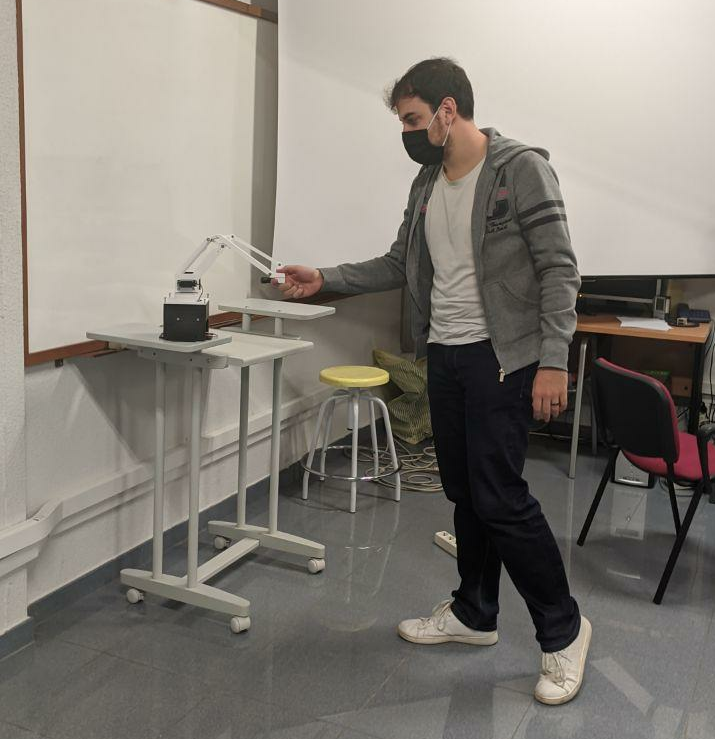
\includegraphics[width=\linewidth]{pictures/bye_javinator.png}
    \end{minipage}
    \hfill
    \begin{minipage}{.32\linewidth}
        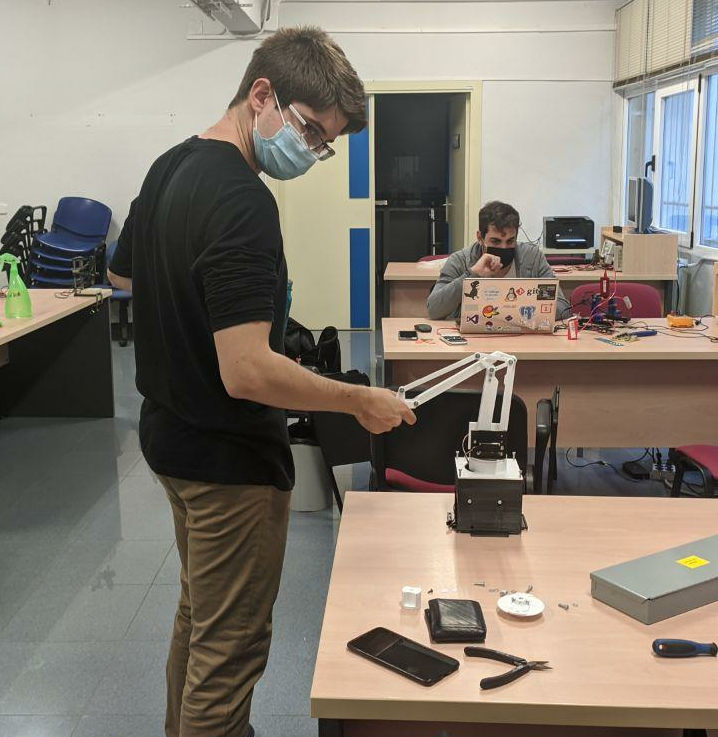
\includegraphics[width=\linewidth]{pictures/bye_mihai.png}
    \end{minipage}
    \hfill
    \begin{minipage}{.32\linewidth}
        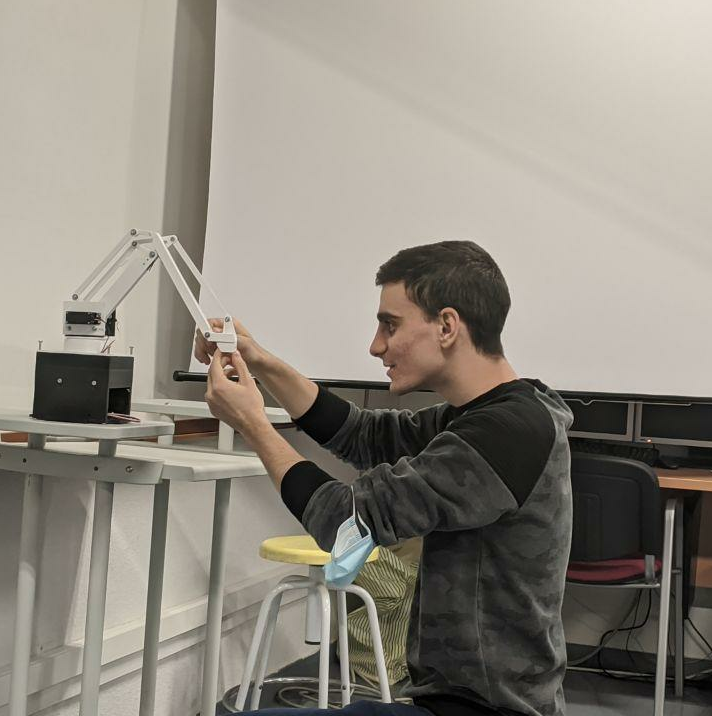
\includegraphics[width=\linewidth]{pictures/bye_alex2.png}
    \end{minipage}
\end{figure}